La figure ci-dessous correspond à la maquette d'un projet architectural.
Il s'agit d'une maison de forme cubique $(ABCDEFGH)$ accolée à un garage de forme cubique $(BIJKLMNO)$ où $L$ est le milieu du segment $[BF]$ et $K$ est le milieu du segment $[BC]$.

Le garage est surmonté d'un toit de forme pyramidale $(LMNOP)$ de base carrée $LMNO$ et de sommet $P$ positionné sur la façade de la maison.

\begin{center}
	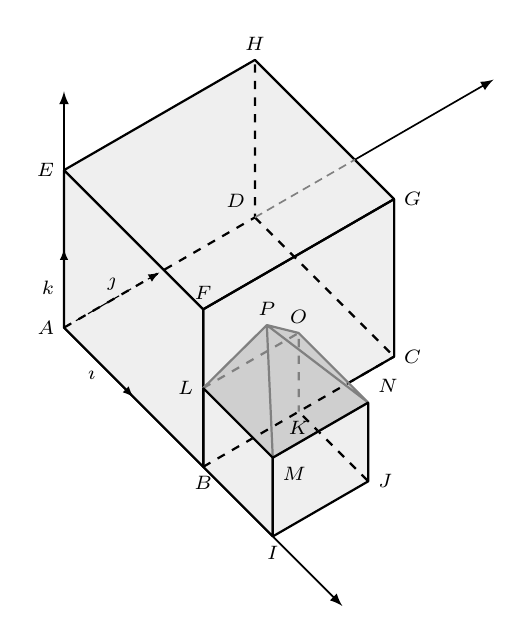
\begin{tikzpicture}[x={(-45:12.5mm)},y={(30:14mm)},z={(90:10mm)},line join=bevel]
		\coordinate (A) at (0,0,0) ;
		\coordinate (B) at (2,0,0) ;
		\coordinate (C) at (2,2,0) ;
		\coordinate (D) at (0,2,0) ;
		\coordinate (E) at (0,0,2) ;
		\coordinate (F) at (2,0,2) ;
		\coordinate (G) at (2,2,2) ;
		\coordinate (H) at (0,2,2) ;
		\coordinate (L) at (2,0,1) ;
		\coordinate (K) at (2,1,0) ;
		\coordinate (I) at (3,0,0) ;
		\coordinate (M) at (3,0,1) ;
		\coordinate (J) at (3,1,0) ;
		\coordinate (N) at (3,1,1) ;
		\coordinate (O) at (2,1,1) ;
		\coordinate (P) at (2,{2/3},{4/3}) ;
		\coordinate (Q) at (2,1.55,0) ;
		\fill[draw=none,semithick,fill=lightgray!25] (A)--(B)--(F)--(E)--cycle ;
		\fill[draw=none,semithick,fill=lightgray!25] (E)--(F)--(G)--(H)--cycle ;
		\fill[draw=none,semithick,fill=lightgray!25] (B)--(C)--(G)--(F)--cycle ;
		\fill[draw=none,semithick,fill=lightgray!25] (B)--(L)--(M)--(I)--cycle ;
		\fill[draw=none,semithick,fill=lightgray!25] (I)--(J)--(N)--(M)--cycle ;
		\fill[draw=none,semithick,fill=lightgray!75] (L)--(M)--(N)--(O)--(P)--cycle ;
		\draw[->,>=latex] (A)--(1,0,0) node[pos=0.4,below=2pt,font=\scriptsize] {$\vect{\imath}$} ;
		\draw[->,>=latex,densely dashed] (A)--(0,1,0) node[midway,above,font=\scriptsize] {$\vect{\jmath}$} ;
		\draw[->,>=latex] (A)--(0,0,1) node[midway,left,font=\scriptsize] {$\vect{k}$} ;
		\draw[thick] (A)--(B)--(F)--(E)--cycle ;
		\draw[thick] (E)--(F)--(G)--(H)--cycle ;
		\draw[thick] (B)--(F)--(G)--(C) ;
		\draw[thick,dashed] (B)--(C) (A)--(D)--(H) (D)--(C) (B)--(K)--(J);
		\draw[thick,gray] (L)--(M)--(N)--(O)--(P)--cycle (P)--(M) (P)--(N) ;
		\draw[thick,gray,dashed] (L)--(O)--(K) ;
		\draw[thick] (B)--(I)--(M)--(L)--cycle (Q)--(C)--(G) ;
		\draw[thick] (I)--(J)--(N)--(M)--cycle ;
		\draw[->,>=latex,semithick] (A)--(4,0,0) ;
		\draw[->,>=latex,semithick] (A)--(0,0,3) ;
		\draw[semithick,gray,densely dashed,] (D)--(0,3.05,0) ;
		\draw[->,>=latex,semithick] (0,3.05,0)--(0,4.5,0) ;
		\foreach \point/\pos in {A/left,B/below,C/right,D/above left,E/left,F/above,G/right,H/above,I/below,J/right,K/below,L/left,M/below right,N/above right,O/above,P/above}
			{\draw (\point) node[font=\scriptsize,\pos] {$\point$} ;}
	\end{tikzpicture}
\end{center}

\smallskip

On munit l'espace du repère orthonormé $\left(A;\vect{\imath},\vect{\jmath},\vect{k}\right)$ avec $\vect{\imath} = \frac12\vect{AB}$, $\vect{\jmath} = \frac12\vect{AD}$ et $\vect{k} = \frac12\vect{AE}$.

\begin{enumerate}
	\item 
	\begin{enumerate}
		\item Par lecture graphique, donner les coordonnées des points $H$, $M$ et $N$.
		\item Déterminer une représentation paramétrique de la droite $(HM)$.
	\end{enumerate}
	\item L'architecte place le point $P$ à l'intersection de la droite $(HM)$ et du plan $(BCF)$.
	
	Montrer que les coordonnées de $P$ sont $\left(2;\frac23;\frac43\right)$.
	\item 
	\begin{enumerate}
		\item Calculer le produit scalaire $\vect{PM}\cdot\vect{PN}$.
		\item Calculer la distance $PM$.
	\end{enumerate}
	On admet que la distance $PN$ est égale à $\frac{\sqrt{11}}{3}$.
	\begin{enumerate}[resume]
		\item Pour satisfaire à des contraintes techniques, le toit ne peut être construit que si l'angle $\widehat{MPN}$ ne dépasse pas \ang{55}. Le toit pourra-t-il être construit ?
	\end{enumerate}
	\item Justifier que les droites $(HM)$ et $(EN)$ sont sécantes. Quel est leur point d'intersection ?
\end{enumerate}
